% Owner: member A. Target length: 1.25 pages.
% Numbers: results/results.csv. Tables and figures: python -m scripts.trend_analysis.
\section{Methods}\label{sec:methods}

All models go through one shared evaluation function. It selects the feature columns, fits the model, scores the holdout and writes one row to a common results log. Every member therefore compares models on the same rows, the same features and the same metrics. The random seed is 5228 for every fit.

\subsection{Validation Design}\label{sec:validation}

The test set lies after the training set in time, so a random split would let a model see rents from the months it is asked to predict. We use a time holdout that copies this situation. Models are fitted on rentals approved from January 2021 to September 2024 (132{,}538 rows) and scored on October 2024 to March 2025 (17{,}037 rows). This follows the usual practice for evaluating forecasts~\cite{hyndman2021forecasting,bergmeir2012use}. Only fit rows are used to compute encodings, imputation values, scalers and the rent index of Section~\ref{sec:trend}.

To show what a random split would have told us, we also run shuffled 5-fold cross-validation (CV) for several models. Random CV covers all months from 2021 to 2025, and the spread of rent differs between months, so its overall RMSE cannot be compared with the holdout RMSE. We therefore score the random CV predictions only on the rows from October 2024 to March 2025. Both numbers then cover the same rows, and their difference measures only the effect of the split. Table~\ref{tab:split} gives the result.

\begin{table}[htbp]
\caption{RMSE (SGD) on the October 2024 to March 2025 rows under the time holdout and under random 5-fold CV. Gap is time minus random.}
\label{tab:split}
\centering
\footnotesize
\begin{tabular}{lrrr}
\hline
\textbf{Model} & \textbf{Time} & \textbf{Random} & \textbf{Gap} \\
\hline
Global median & 837.1 & 794.6 & +42.5 \\
Group median & 754.9 & 490.5 & +264.4 \\
Linear regression & 575.4 & 502.2 & +73.2 \\
Ridge & 576.1 & 502.7 & +73.3 \\
KNN & 482.3 & 508.6 & -26.3 \\
Decision tree & 482.9 & 480.6 & +2.3 \\
Random forest & 458.7 & 461.1 & -2.4 \\
Random forest + index & 444.3 & 451.9 & -7.6 \\
LightGBM (default) & 457.3 & 455.3 & +2.0 \\
CatBoost (default) & 452.7 & 451.6 & +1.2 \\
XGBoost (default) & 457.2 & 456.5 & +0.7 \\
LightGBM (tuned) & 449.9 & 451.9 & -2.0 \\
LightGBM (tuned) + index & 445.8 & 450.7 & -4.9 \\
CatBoost (tuned) & 448.8 & 451.0 & -2.1 \\
XGBoost (tuned) & 449.9 & 450.8 & -0.9 \\
\hline
\end{tabular}

\end{table}

Random CV does not flatter the tree models: their gap lies between $-8$ and $+2$~SGD. It does flatter the models that handle time poorly. The group median gains 264~SGD from a random split, because random folds contain fit rows from the same calendar quarters as the validation rows, so the lookup can use the exact quarter instead of falling back to medians over all past months. Linear regression and Ridge gain 73~SGD, because a random split hides the error of extending a straight time trend into new months. A model choice made with random CV would therefore have overrated the simple models. The time holdout is the only one of the two splits that matches the test situation, and all other results in this report use it.

The final model was tuned and selected on this same holdout, so its holdout RMSE is slightly optimistic. We did not hold out a second period, because it would have removed the most recent months from training.

\subsection{Metrics}

Kaggle ranks submissions by the root mean squared error (RMSE), so RMSE is our primary metric. We also report the mean absolute error (MAE), the mean absolute percentage error (MAPE) and the bias, defined as the mean prediction minus the mean observed rent. The bias shows whether a model follows the rent level. For the time holdout we also compute RMSE per validation month and per flat type.

\subsection{Feature Groups}\label{sec:groups}

We split the features into four fixed groups and use the same groups in every experiment:
\begin{itemize}
\item \textbf{G0 core} (13 features): town, flat type and its ordinal, flat model, floor area and two transforms of it, lease year, flat age, an invalid lease flag, and the month index with a cyclic month.
\item \textbf{G1 location} (26): block latitude and longitude, subzone, distance to the central business district, and distances and counts within 0.5 to 2~km for MRT stations (open and planned), schools, primary schools, malls, rail lines and tertiary campuses.
\item \textbf{G2 block} (5): maximum floor, completion year and age of the block, with two missing value flags.
\item \textbf{G3 market} (10): COE premiums and demand ratios, CPI and stock market values for the approval month.
\end{itemize}
All baselines use G0+G1 (39 features) unless stated otherwise. The ablation in Section~\ref{sec:evaluation} adds and removes whole groups. The G3 values would not be known at the time of a real forecast, so we only use them to test whether they help.

\subsection{Trend Handling}\label{sec:trend}

Tree models predict the average target of a leaf, so they cannot predict a rent above the highest level they saw in training. If rents keep rising after the last training month, a tree model fitted on raw rent will predict too low for later months. We compare two ways to handle the trend:
\begin{itemize}
\item \textbf{Raw}: the model predicts the rent directly. The month index is one of its features.
\item \textbf{Index}: the model predicts the ratio of the rent to a monthly rent index, and the prediction is multiplied back by the index.
\end{itemize}
For a month $t$ inside the fit period, the index $I_t$ is the median rent of the fit rows approved in month $t$. For a later month, $I_t$ comes from a straight line fitted by least squares to the last 12 monthly medians of the fit period. A model $f$ is trained on $y_i / I_{t_i}$ and predicts
\begin{equation}
\hat{y}_i = f(x_i)\, I_{t_i}.
\end{equation}
The line is fitted on fit rows only, so the index uses no information from the holdout months. The model still receives the month index as a feature, so it can learn changes in the rent ratio over time. Fig.~\ref{fig:index} shows the index. Rents rose quickly in 2022 and 2023 and were nearly flat from February 2024, so the extrapolated index rises by only about 2.4~SGD per month. In the six holdout months it stays within 73~SGD of the observed median (mean difference $-16$~SGD).

\begin{figure}[htbp]
\centerline{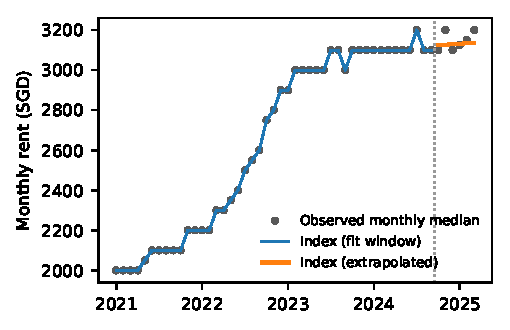
\includegraphics[width=\columnwidth]{figures/rent_index}}
\caption{Monthly median rent and the rent index fitted on January 2021 to September 2024. After the dotted line the index is extrapolated.}
\label{fig:index}
\end{figure}

\begin{table}[htbp]
\caption{Time holdout RMSE (SGD) with the raw target and the index target, G0+G1 features. Change is index minus raw.}
\label{tab:trend}
\centering
\footnotesize
\begin{tabular}{lrrr}
\hline
\textbf{Model} & \textbf{Raw} & \textbf{Index} & \textbf{Change} \\
\hline
Global median & 837.1 & 641.5 & $-195.6$ \\
Group median & 754.9 & 483.1 & $-271.8$ \\
Linear regression & 575.4 & 467.6 & $-107.8$ \\
Ridge & 576.1 & 467.9 & $-108.2$ \\
KNN & 482.3 & 481.9 & $-0.4$ \\
Decision tree & 482.9 & 473.3 & $-9.7$ \\
Random forest & 458.7 & 444.3 & $-14.4$ \\
LightGBM (default) & 457.3 & 454.3 & $-3.0$ \\
CatBoost (default) & 452.7 & 452.2 & $-0.5$ \\
XGBoost (default) & 457.2 & 459.6 & $+2.4$ \\
LightGBM (tuned) & 449.9 & 445.8 & $-4.1$ \\
CatBoost (tuned) & 448.8 & 449.0 & $+0.2$ \\
XGBoost (tuned) & 449.9 & 445.6 & $-4.3$ \\
\hline
\end{tabular}

\end{table}

Table~\ref{tab:trend} shows that the index target lowers the RMSE of 11 of the 13 models. Tuned CatBoost changes by 0.2~SGD. Default XGBoost gets 2.4~SGD worse, but tuned XGBoost gains 4.3~SGD. The gain is largest for the models that cannot represent the rent level well on their own. The global and group medians improve by 196 and 272~SGD, because their raw predictions are medians over all fit months and lie more than 500~SGD below the holdout rents. Linear regression and Ridge improve by 108~SGD. On raw rent they over-predict by 330~SGD on average, because the month coefficient learns the steep rise of 2022 and 2023 and extends it into a period when rents had stopped rising. The other tree models improve by 0 to 14~SGD. They already use the month index to separate recent rows from old ones, but each leaf still averages some older and cheaper rows, so their raw predictions are 28 to 50~SGD too low on average. The index target reduces this bias. With the index target, the untuned random forest (444.3~SGD), tuned XGBoost (445.6~SGD) and tuned LightGBM (445.8~SGD) are the three best models. They lie within 1.5~SGD of each other. The index also removes most of the gap between the simple and the complex models: Ridge falls from 126 to 22~SGD behind LightGBM.

\begin{figure*}[htbp]
\centerline{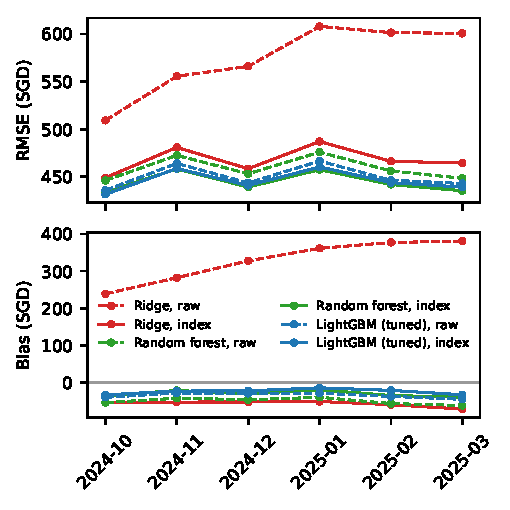
\includegraphics[width=\textwidth]{figures/monthly_rmse}}
\caption{RMSE (left) and bias (right) per validation month for three models, with the raw target (dashed) and the index target (solid).}
\label{fig:monthly}
\end{figure*}

Fig.~\ref{fig:monthly} shows the error per holdout month. For the tree models the error does not grow from October 2024 to March 2025, and the index target lowers it by a similar amount in every month. For Ridge on raw rent the bias grows from 239 to 381~SGD over the six months, which is the expected sign of a wrong trend. Because rents were nearly flat in the holdout period, this holdout cannot show how well a tree model follows a trend that keeps rising. The test period extends up to 16 months past the training data, and only the index target lets a tree model predict a rent level it has not seen. We therefore use the index target for the final model.

\subsection{Models}\label{sec:models}

We compare models in order of complexity, all on the same split and features:
\begin{enumerate}
\item \textbf{Global median} of the fit rows, as a lower bound.
\item \textbf{Group median}: the median rent per town, flat type and calendar quarter. If a group has no fit rows, the lookup falls back to town and flat type, then flat type, then town.
\item \textbf{Linear regression} and \textbf{Ridge} ($\alpha = 10$) with one-hot town, flat type, flat model and subzone. As noted in the progress report, area and flat type are strongly related, so these models keep flat type and drop the area columns.
\item \textbf{$k$-nearest neighbours} ($k = 50$, distance weights) on scaled latitude, longitude, floor area and month.
\item \textbf{Decision tree} (depth 16, at least 20 rows per leaf).
\item \textbf{Random forest}~\cite{breiman2001random} (300 trees, depth 20, at least 5 rows per leaf, 70\% of the features per split).
\item \textbf{LightGBM}~\cite{ke2017lightgbm}, \textbf{CatBoost}~\cite{prokhorenkova2018catboost} and \textbf{XGBoost}~\cite{chen2016xgboost}, gradient boosted trees with native handling of categorical features, first with default settings and then tuned.
\end{enumerate}
The baselines use scikit-learn~\cite{pedregosa2011scikit}. Their settings are fixed and were not tuned.

\subsection{Tuning Budget}

We gave each of the three boosting models a fixed budget of 30 trials of Optuna~\cite{akiba2019optuna} with the tree-structured Parzen estimator~\cite{bergstra2011algorithms}, minimising the time holdout RMSE with G0+G1 features and the raw target. The search covers the number of trees, learning rate, tree size, row and feature subsampling and regularisation (Appendix~\ref{app:hyperparameters}). The tuned settings are then held fixed for the ablations and for the index target. We stopped when the budget ran out, because the course feedback warned against chasing small RMSE gains.
